\section{Results}
\label{sec:results}

The results of the main project I implemented
during my three-month internship at isMOOD can be divided
into three main categories:

\begin{itemize}
  \item \emph{Phase 1: Research Conduction}: It includes all research that was conducted
  in order to find the most suitable approach
  that would be followed for the accomplishment of the project. 
  \item \emph{Phase 2: Database Construction}: It includes all activities related to the construction
  of the database.
  \item \emph{Phase 3: Algorithm Development}: It summarises all activities related to the development
  of the algorithm in Python.
\end{itemize}

Courses of the University that contributed to the fulfilment
of the activities of the above phases are the following:

\begin{itemize}
 \item Algorithms and Data Structures (Semester 4)
 \item Database Management Systems (Semester 3)
 \item Programming I \& II (Semesters 2 \& 3)
 \item Software Engineering in Practice (Semester 6)
 \item Big Data Management Systems (Semester 8)
\end{itemize}

These courses provided me with fundamental knowledge and experience
with Python, databases, and programming in general.

\subsection{Phase 1: Research Conduction}
\label{subsec:research}

To find what approach we would follow,
which are currently the best practices, tools and technologies available
that we would use for the construction of the database
and for the development of the algorithm,
I devoted a two-week time to perform research.

In order to familiarise with the areas
of Text Analytics and Sentiment Analysis,
due to my lack of any previous experience and knowledge on them,
I searched on Google Scholar\footnote{\url {https://scholar.google.gr/}}
for associated research.
At first, my research was not language specific
because my intention was to understand these areas.
Luckily, a variety of studies are publicly available
and I was provided with a lot of information.

From my initial research, I found that 
there are currently two main approaches
to perform Sentiment Analysis in Software Engineering.
The first approach uses Machine Learning methods.
It facilitates from already available data,
however there is one critical restriction.
The algorithm that uses Machine Learning methods
is usually trained on data from specific domains,
thus when a new domain is introduced,
the algorithm usually does not perform adequately well.
isMOOD already uses this approach
and is challenged by the abovementioned downside,
and for that reason they asked me to develop
an algorithm based on the second approach.
This approach would be used on untrained domains of data.

The second approach to perform Sentiment Analysis
can be characterised as a more general approach.
It uses a lexicon as its base (lexicon-based)
which contains terms annotated with sentiment,
receives a text as input, divides it into words,
and each word is mapped to the lexicon
in order to find its sentiment.
In its simplest form, the one I also implemented,
the overall sentiment of the text is inferred
through the aggregate-and-average method,
as explained in the thorough guide
to lexicon-based methods for sentiment analysis~\cite{TBTV11};
we sum the sentiment (positive, negative, objective) scores
of all words and divide them with the total number of words.
The preponderant sentiment that occurs in this way
is the final overall text sentiment.

The problem with this approach is that it is language dependent
since it requires a lexicon of terms annotated with sentiment.
From my research, I unfortunately discovered that there are
not enough annotated sources of data for the Greek language.
In order to solve this issue
and generate the required annotated Greek lexicon for our project,
we decided to translate an English annotated lexicon to Greek.

For that purpose I searched and found
that the best publicly available English annotated lexicon
is SentiWordNet 3.0.\footnote{\url {https://github.com/aesuli/SentiWordNet}}
For the translation, I found that the most appropriate translator
is the Google Cloud Translation API.\footnote{\url {https://cloud.google.com/translate/docs/}}
The downside of Google Cloud Translation API is
that it is not free.
Despite that, when you create a new Google Cloud account
you are currently provided with a free amount of credits
that you can use on any available Google service.
The amount provided was sufficient to translate all terms
included in SentiWordNet 3.0 without being further charged.

The default limits of Google Cloud Translation API\footnote {\url {https://cloud.google.com/translate/quotas}} were modified as follows:

\begin{itemize}
 \item 10,000,000 characters per 100 seconds (per user)
 \item 1,000 requests per 100 seconds (per user)
\end{itemize}

For the development of the algorithm,
I was instructed to create a simple algorithm, a baseline.
From the research that was conducted and after a lot of fruitful discussions
with all the professionals mentioned
in Section~\ref{subsec:technical-activities},
it was decided to use lemmatisation on words that were not directly mapped
to the Greek annotated lexicon,
and then use the average-and-aggregate method
for the calculation of the overall text sentiment.
For the lemmatisation, it was discovered
that the best available lemmatiser in Python
adapted to the Greek language is provided
by the spaCy library.\footnote{\url {https://spacy.io/models/el}}

\subsection{Phase 2: Database Construction}
\label{subsec:database}

\subsubsection{Implementation}
\label{subsubsec:dbimplementation}

MongoDB 3.4 was used to store the database.
The most time consuming process of the project
was the construction of the particular database;
this process took almost two months.
There are three main reasons for that.

The first reason lies in the multiple reconstructions
that were made to the database schema;
the schema changed more than five times.
What I learned in practice and what my supervisor informed me is
that as you build a database,
the schema matures in your mind,
and as you process the information stored,
you find more efficient ways to represent it in the schema.

The second reason lies in the time consuming queries
that were run in order to store all information.
All queries to MongoDB were run through OpenVPN
on a 6-core Cloud Virtual Machine with 16GB RAM
provided by DigitalOcean.
The queries were executed far more quickly in this way
than on a local computer, plus they could be run
in screen mode, thus have parallel executions of multiple queries,
without worrying about any interruptions
that would lead to the failure of a query.

Despite that, some queries would run for days.
For instance, the population of the Greek lexicon with the lemmas
produced from it took five days.
Furthermore, the sentiment mapping from the translated terms
of SentiWordNet 3.0. to the terms of the Greek lexicon
required two days.
What is more, some time consuming queries, like the sentiment mapping,
had to be executed repeatedly as the database schema changed,
in order to ensure consistency and validity for the data.

In addition,
the fact that the Technical team often made critical changes and updates
to MongoDB that required for MongoDB to be restarted urgently
while some queries were executed at the same time,
would lead to the untimely termination of them.
Some of them were not possible to continue
from the point they had stopped,
thus had to run from the beginning again.

The third reason behind the time consuming construction of the database
is related to the complex information that was stored.
A lot of sources were combined and used to gather information,
and multiple processes were performed on them
to transform the information in the desired format
and then produce extra attributes.

At the end, the final database schema in MongoDB
that we named ``lexicondb''
is composed of four collections,
as depicted in the following figure,
and they are all explained in detail.
Statistics of the collections are also included,
along with an example of a record.

\begin{figure}[ht]
\centering
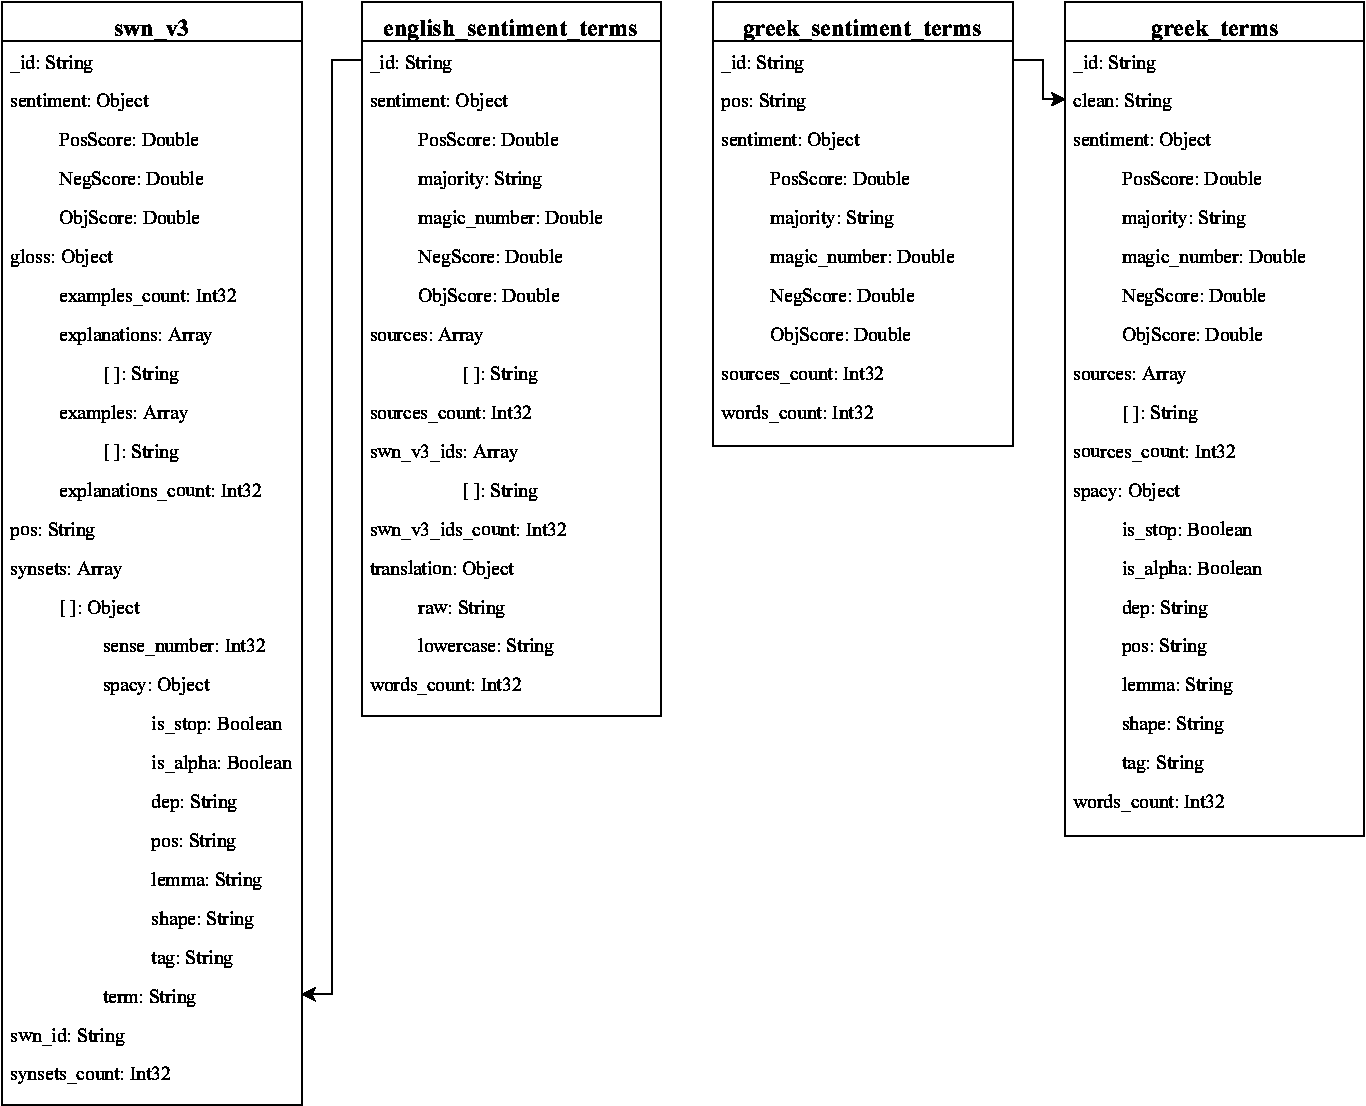
\includegraphics[width=\textwidth]{mongodb-schema.eps}
\caption{MongoDB Database Schema -- lexicondb}
\label{fig:mongodb-schema}
\end{figure}

\clearpage

\subsubsubsection{swn\_v3}
\label{subsubsubsec:swn-v3}

This is the first collection that was created.
It contains all records of SentiWordNet 3.0.
The data of the source file that is publicly available\footnote{\url {https://github.com/aesuli/SentiWordNet/blob/master/data/SentiWordNet_3.0.0.txt}}
and that was used are in a complex format,
making it the most difficult data source that had to be parsed
for the construction of the particular database.
The source file was initially converted
from text (txt) format to comma-separated-values (csv) format,
and all comments included in the file were removed
to make it parsable.

While parsing it with a Python script, it was discovered that
some fields do not always follow a standard pattern.
All troubled fields were manually inspected
in order to detect all possible patterns that were followed.
Then multiple checks and filters were applied to the Python script 
according to the detected patterns,
in order to construct the particular collection,
based on a standard format.
We finally formed the following fields:

\begin{itemize}
  \item \emph{\_id}: A concatenation of the ``pos'' (part-of-speech)
  and the ``id'' fields of the source file.
  This is the unique id of each record according to the SentiWordNet 3.0
  documentation provided in the beginning of the source file. 
  
  \item \emph{sentiment}: It includes the fields ``PosScore'' (Positive Score)
  and ``NegScore'' (Negative Score).
  The field ``ObjScore'' (Objective Score) is calculated
  based on the following formula according to the documentation: \\
  $ObjScore = 1 - (PosScore + NegScore)$
  
  \item \emph{gloss}: The most troubled field.
  It includes explanations and examples of the use of the synonym sets
  of the particular record.

  For the examples, we noticed that they start with quotation marks
  and initially distinguished them based on that.
  We later found that some examples also include other phrases 
  in quotation within them (e.g. ``the word `dog' is animate'')
  and this was not initially covered by our filters,
  leading in some cases to wrong inputs to the field ``examples''.
  In the above example, there would be inserted three examples
  instead of one: ``the word'', ``dog'', ``is animate''.
  We fixed this by applying regex rules
  that bypassed the inside quotation marks.

  For the explanations, we simply checked for a phrase
  whether it was an example according to the above rules,
  and if not, then is was an explanation.
  All phrases are separated by a semicolon (``;'')
  and we used this as a delimiter to separate the phrases
  of each record.
  We also included the number of explanations and examples
  found in the particular record.
  
  \item \emph{pos}: The part-of-speech of the record.
  
  \item \emph{synsets}: One major difference between SentiWordNet 3.0
  and 1.0 (the previous version) is
  that 3.0 follows the ``bag-of-synsets'' logic
  instead of ``bag-of-words'' that is followed in 1.0~\cite{BES10}.
  This means that each record contains multiple terms
  that are semantically associated (synonym sets).
  
  For each record, we separated all terms included,
  and made an object for each term under ``synsets''.
  Each ``term'' contains a ``sense\_number'' from the source file,
  which is a number that indicates the relevance of the term
  to the particular synonym set, starting with a hashtag (``\#'').
  In addition, we used spaCy library
  to derive more grammatical information~\footnote{\url {https://spacy.io/usage/linguistic-features}}
  about each term, and placed it under the field ``spacy''.
  
  \item \emph{swn\_id}: The id included in the source file for each record.
  However, this id is not unique.
  
  \item \emph{synsets\_count}: The number of terms
  found in the particular synonym set.
\end{itemize}

\subsubsubsection{english\_sentiment\_terms}
\label{subsubsubsec:english-sentiment-terms}

After constructing swn\_v3,
we constructed a second collection
with the unique terms found in SentiWordNet 3.0 as ids.
What was noticed is that some terms are included
in multiple synonym sets;
for these, the sentiment scores are averages
(the scores of all occurrences of a term were summed
and divided with the number of occurrences),
rounded to three decimal places.
The fields included in this collection are the following:

\begin{itemize}
 \item \emph{\_id}: A unique term of swn\_v3.

 \item \emph{sentiment}: It contains the average sentiment scores
 (``PosScore'', ``NegScore'', ``ObjScore'') computed as described above
 and rounded to three decimal places.
 It also includes the preponderant sentiment based on the maximum score
 (field ``majority'').

 ``magic\_number'' is a number that occurred after a lot of hours
 of discussion with my colleagues of the Technical team.
 We wanted to produce a number that would indicate for a term
 how strongly annotated it is
 (i.e. how much difference there is among its sentiment scores).
 At the end, we came up with the following formula: \\
 $magic\_number = (max\_score - intermediate\_score) + (max\_score - min\_score)$ \\
 This number receives values in range $[0,2]$.
 
 \item \emph{sources}: It includes all ids of the swn\_v3 records
 where the particular term was found.
 
 \item \emph{sources\_count}: The number of the above record ids.
 
 \item \emph{translation}: The translation of the term in Greek
 based on the Google Cloud Translation API
 as described in Section~\ref{subsec:research}.
 Two versions of the translation are included:
 the raw translation and the translation in lowercase.
 The second is used to match a translation of an English term
 to a Greek term of greek\_terms in order to transfer sentiment,
 excluding any case sensitivity.
 
 \item \emph{words\_count}: Some terms are phrases, thus
 it is listed for each term how many words it is composed of.
\end{itemize}

\subsubsubsection{greek\_terms}
\label{subsubsubsec:greek-terms}

For the creation of the Greek lexicon,
three initial data sources were used:

\begin{enumerate}
 \item \emph{Aspell v0.08}: An official Greek dictionary used in OpenOffice/LibreOffice Spell~\footnote{\url {http://www.elspell.gr/myspell}}
 that contains 828,806 terms.
    
 \item \emph{Wiktionary}: A dictionary of 92,747 Greek terms from Wiktionary.~\footnote{\url {https://github.com/eellak/gsoc2018-spacy/blob/6212c56f94ca3926b0959ddf9cee39df28e1c5a8/spacy/lang/el/lemmas/elwords_from_wiktionary.txt}}

 \item \emph{Greek Lemmas}: A collection of 458,331 Greek terms with their lemmas
 from the Google Summer of Code 2018 - 3gm project.~\footnote{\url {https://github.com/eellak/gsoc2018-3gm/blob/master/resources/greek_lemmas.py}}
\end{enumerate}

The dictionary was then populated with the lemmas of the terms
derived from spaCy library, leading to 97,793 new records in the collection.
Eventually the following fields were constructed:

\begin{itemize}
 \item \emph{\_id}: A unique term derived from one of the above data sources.
 
 \item \emph{clean}: The term in lowercase with no intonation.
 
 \item \emph{sentiment}: The sentiment mapped from english\_sentiment\_terms
 based on the lowercase translation.
 If the term was found in multiple lowercase translations,
 then the average scores are computed and inserted,
 rounded to three decimal places.
 The preponderant sentiment that corresponds to the maximum sentiment score
 is also included, along with the magic number as described before.
 
 \item \emph{sources}: The data source(s) of the term:
 ``aspell'', ``wiktionary'', ``greek\_lemmas'', ``lemmas\_generated''.
 
 \item \emph{sources\_count}: The number of data sources of the term.
 
 \item \emph{spacy}: Grammatical information of the term
 derived from spaCy library.
 
 \item \emph{words\_count}: The number of words that the term is composed of.
\end{itemize}

\subsubsubsection{greek\_sentiment\_terms}
\label{subsubsubsec:greek-sentiment-terms}

The last collection that was created
contains the clean terms of greek\_terms as ids.
The reason lies in the algorithm,
as described in Section~\ref{subsec:algorithm};
the input text is cleaned from any case sensitivity or intonation,
thus a clean version of the Greek lexicon was needed
in order to match the words of the input text to the words of the lexicon.

This collection contains only words ($words\_count = 1$)
that have received sentiment through the process
described in Section~\ref{subsubsubsec:greek-terms}.
If a clean word was found in multiple records of greek\_terms,
again the average scores are computed and inserted
to the ``sentiment'' field,
rounded to three decimal places.
The fields of this collection are listed below:

\begin{itemize}
 \item \emph{\_id}: A unique clean term from greek\_terms.
 
 \item \emph{pos}: The part-of-speech of the term.
 In cases of multiple occurrences of a clean term in greek\_terms,
 the part-of-speech receives the preponderant value,
 by counting the frequences of each part-of-speech
 and computing the maximum value.
 
 \item \emph{sentiment}: The sentiment of the clean term.
 Again in multiple occurrences of the clean term,
 the average scores are computed and inserted,
 rounded to three decimal places.
 
 \item \emph{sources\_count}: The number of occurrences
 of the clean term in greek\_terms.
 
 \item \emph{words\_count}: Since only single words are included,
 this field always has the value ``1''.
\end{itemize}

\subsubsection{Statistics}
\label{subsubsec:statistics}

The number of records of each collection is listed below:

\begin{itemize}
 \item \emph{swn\_v3}: 117,659 records
 \item \emph{english\_sentiment\_terms}: 148,834 records
 \begin{itemize}
  \item 4,869 with positive preponderant sentiment
  \item 7,269 with negative preponderant sentiment
  \item 136,696 with objective preponderant sentiment
 \end{itemize}
 \item \emph{greek\_terms}: 951,755 records
 \begin{itemize}
  \item 132,943 unique from Aspell
  \item 6,399 unique from Wiktionary
  \item 55 unique from Greek Lemmas
  \item 97,793 new terms (lemmas) produced from spaCy library
  \item 427,233 from two sources (Aspell/Wiktionary/Greek Lemmas/Lemmas Generated)
  \item 271,124 from three sources
  \item 16,208 from four sources
 \end{itemize}
 \item \emph{greek\_sentiment\_terms}: 27,542 records
 \begin{itemize}
  \item 1,252 with positive preponderant sentiment
  \item 1,883 with negative preponderant sentiment
  \item 24,407 with objective preponderant sentiment
 \end{itemize} 
\end{itemize}

To the best of our knowledge,
the collection ``greek\_sentiment\_terms'' currently forms
the largest publicly available Greek lexicon annotated with sentiment.

\subsubsection{Example of Record}
\label{subsubsec:recexample}

In the following figures
the Greek term ``\textgreek{kakos}'' occurred in greek\_sentiment\_terms
from the term ``\textgreek{kak'os}'' of greek\_terms.
The terms ``maleficent'' and ``wicked'' of english\_sentiment\_terms
are translated as ``\textgreek{kak'os}''.
``maleficent'' was found in one record in swn\_v3,
whereas ``wicked'' was found in five records. \\

\textbf{greek\_sentiment\_terms: \textgreek{kakos}} \\

\begin{figure}[ht]
\centering
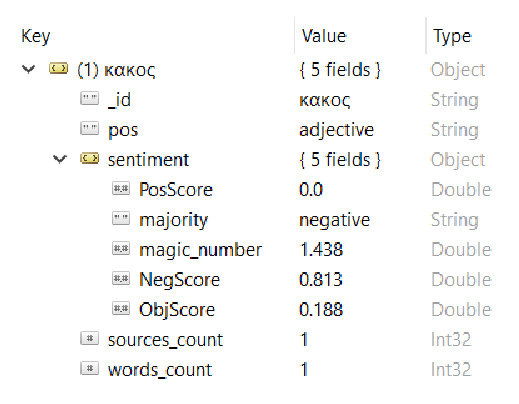
\includegraphics{record/greek-sentiment-terms-kakos.eps}
\caption{greek\_sentiment\_terms -- Example}
\label{fig:gst-kakos}
\end{figure}

\clearpage

\textbf{greek\_terms: \textgreek{kak'os}} \\

\begin{figure}[ht]
\centering
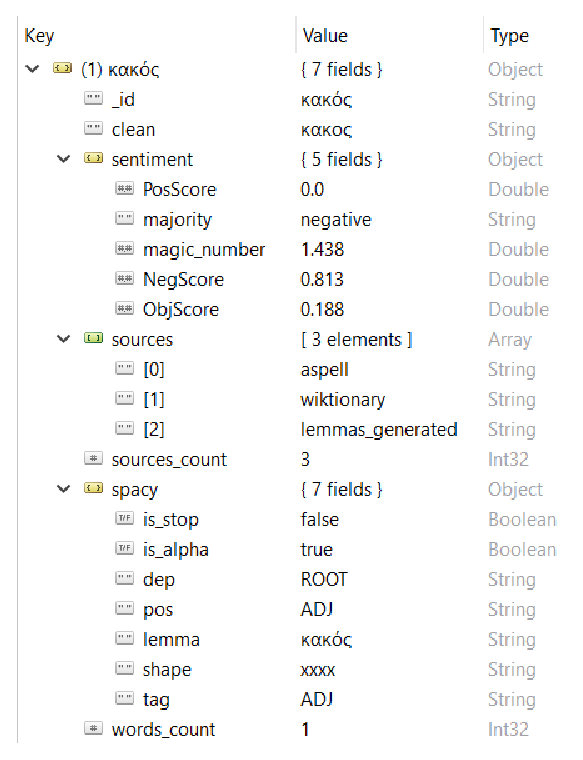
\includegraphics{record/greek-terms-kakos.eps}
\caption{greek\_terms -- Example}
\label{fig:gt-kakos}
\end{figure}

\clearpage

\textbf{english\_sentiment\_terms: maleficent} \\

\begin{figure}[ht]
\centering
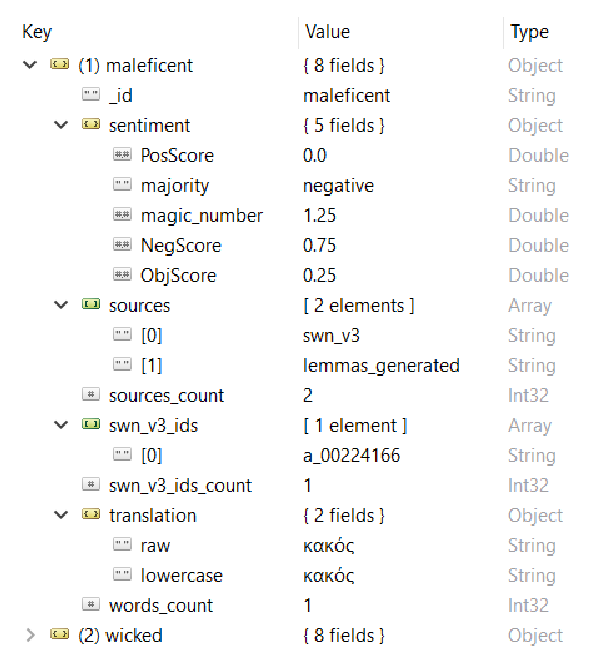
\includegraphics{record/english-sentiment-terms-maleficent.eps}
\caption{english\_sentiment\_terms -- Example 1}
\label{fig:est-maleficent}
\end{figure}

\clearpage

\textbf{english\_sentiment\_terms: wicked} \\

\begin{figure}[ht]
\centering
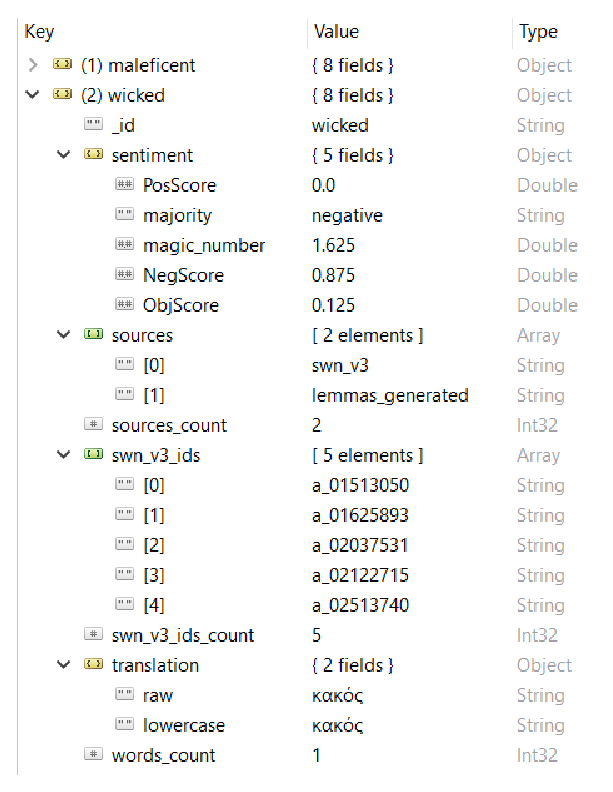
\includegraphics{record/english-sentiment-terms-wicked.eps}
\caption{english\_sentiment\_terms -- Example 2}
\label{fig:est-wicked}
\end{figure}

\clearpage

\textbf{swn\_v3: maleficent} \\

\begin{figure}[ht]
\centering
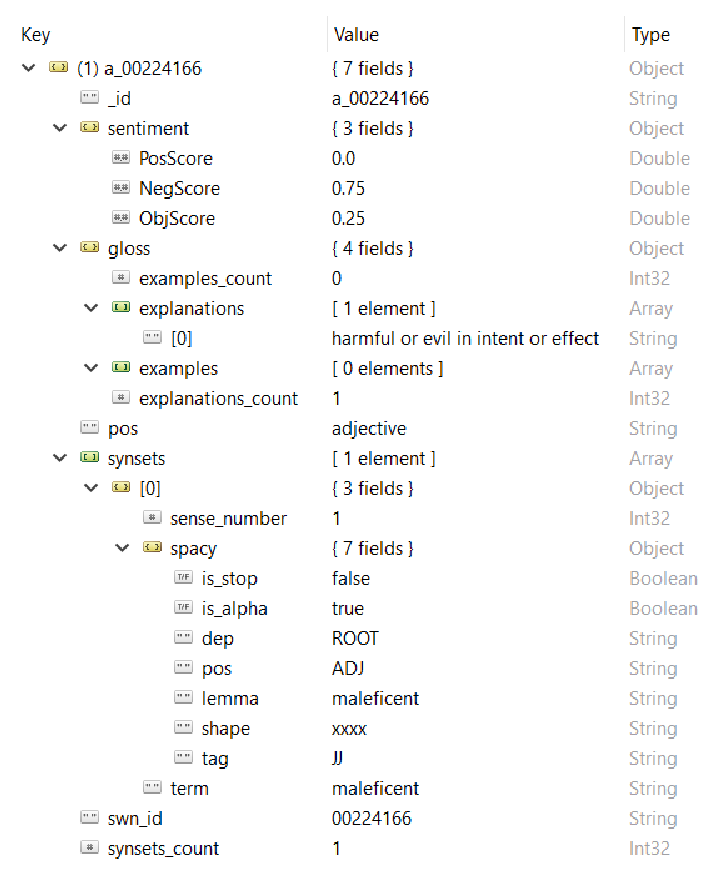
\includegraphics{record/swn-v3-maleficent.eps}
\caption{swn\_v3 -- Example 1}
\label{fig:swn-maleficent}
\end{figure}

\clearpage

\textbf{swn\_v3: wicked} \\

\begin{figure}[ht]
\centering
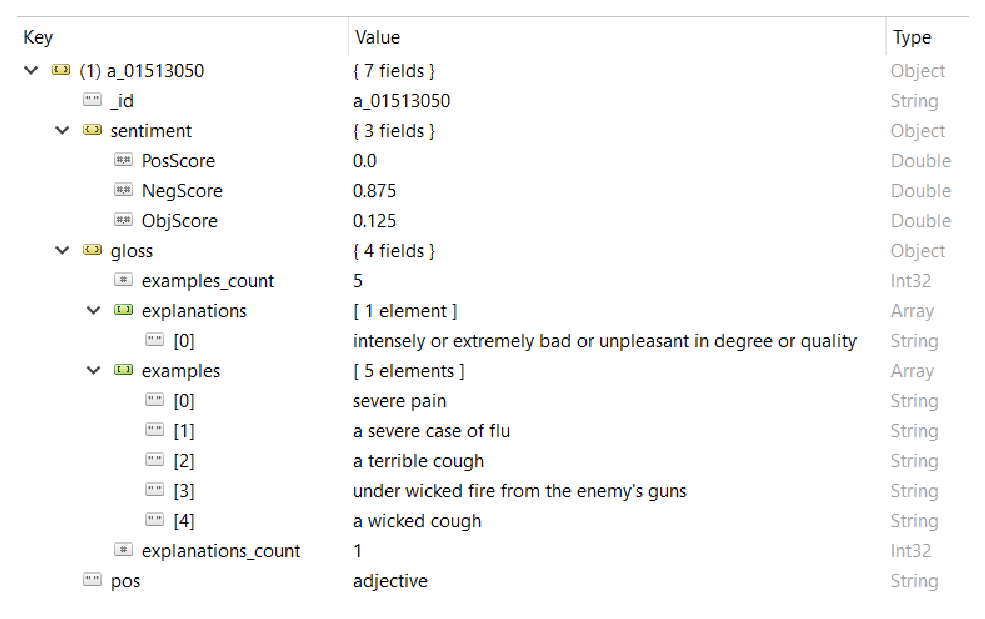
\includegraphics{record/swn-v3-wicked.eps}
\caption{swn\_v3 -- Example 2a}
\label{fig:swn-wicked}
\end{figure}

\clearpage

\textbf{swn\_v3: wicked} \textit{(continues)} \\

\begin{figure}[ht]
\centering
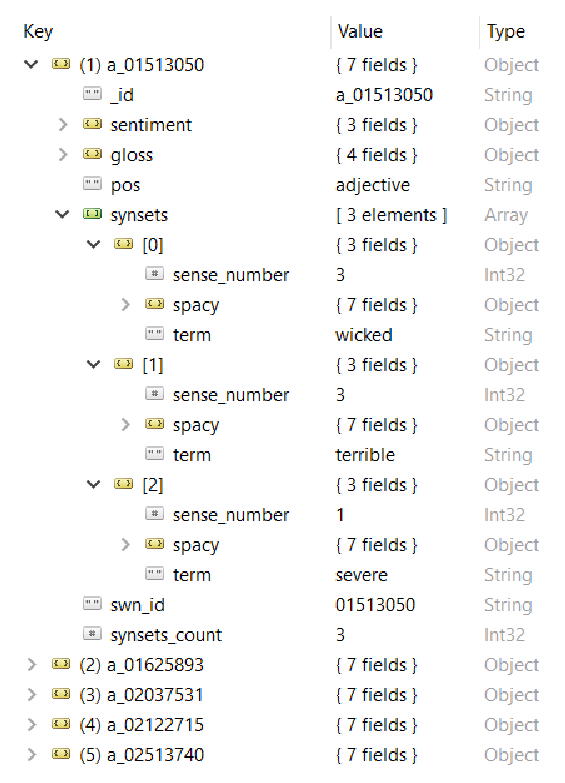
\includegraphics{record/swn-v3-wicked(2).eps}
\caption{swn\_v3 -- Example 2b}
\label{fig:swn-wicked2}
\end{figure}

\clearpage

\subsection{Phase 3: Algorithm Development}
\label{subsec:algorithm}

\subsubsection{Implementation}
\label{subsubsec:algimplementation}

The algorithm was developed in Python 2.7
according to the aggregate-and-average method,
as stated in Section~\ref{subsec:research}.
The development began before the database was finalised,
and was completed in four weeks' time.

The algorithm starts by initialising a dictionary
with the terms of greek\_sentiment\_terms,
along with their sentiment (positive, negative, objective) scores.
A text of type String is received as input.
The text is separarated into sentences
and each sentence is then cleaned from the following features:

\begin{itemize}
 \item the ``RT'' notation that is found in Twitter posts
 \item hashtags that start with the symbol ``\#''
 \item mentions of users that start with the symbol ``@''
 \item links
 \item numbers
 \item stop words derived from a pre-defined list
 \item punctuation
 \item intonation
 \item uppercase: All characters are converted to lowercase.
 \item non-alphanumeric characters
 \item identical consecutive characters:
 No more than one identical consecutive vowel
 or two identical consecutive consonants are allowed in a word;
 any extra vowels/consonants are removed from the word
 (e.g. ``\textgreek{paiizw}'' becomes ``\textgreek{paizw}'',
 ``\textgreek{kuparisssi}'' becomes ``\textgreek{kuparissi}'').
\end{itemize}
A particular script of isMOOD is used for the text cleaning,
unfortunately not publicly available.

After a sentence is cleaned, it is separated into words.
Each word is first attempted to be matched
to a term of the abovementioned dictionary of greek\_sentiment\_terms.
If it is matched,
the sentiment scores of the particular word are inferred from the dictionary.
If it is not matched to any term of the dictionary,
it is then lemmatised through spaCy library,
using the ``el\_core\_news\_md'' pre-trained statistical model for Greek.\footnote{\url {https://spacy.io/models/el#el_core_news_md}}
The medium model was preferred to the small one,
due to its higher Syntax and Named Entity Recognition (NER) accuracies,
as reported in the Greek Models' Documentation page (\textit {see footnote}).

A second attempt is performed to match the lemma of the word
to a term of the dictionary of greek\_sentiment\_terms.
Again if it matched,
the sentiment scores are derived from the dictionary.
Otherwise, the word is ignored and the next word of the sentence is proceeded
and analysed according to the same process.

When the analysis of all words of a sentence is completed,
the sentiment scores of all words of the particular sentence
are summed and divided with the total number of words.
In this way,
the average sentiment scores of the sentence are computed.

The particular process is repeated for all sentences of the input text.
At the end,
the sentiment scores of all sentences are summed
and divided again with the total number of sentences.
Thus, the final sentiment scores are the averages of the averages.

The final sentiment polarity (positive/negative/objective)
applied to an input text
is derived from the preponderant (maximum) sentiment score.
In case of equal preponderant scores,
priority is conceded first to negative,
then to positive, and lastly to objective sentiment.

The reason behind this bias is explained
from a business perspective.
From the experience of the employees of isMOOD,
clients usually look first at the negative posts
and pay more attention to these
than to the positive or the objective.
In addition, clients tend to complain more
about false positives than false negatives.
Businesswise, it is more serious for a client
to classify the phrase ``\emph{the company X is terrible}'' as positive
than to classify the phrase ``\emph{the company X is great}'' as negative.

\subsubsection{Examples of Execution}
\label{subsubsec:algexample}

In the following figures
a Greek text is inserted in the algorithm as input,
and the preponderant sentiment is calculated,
according to the average text sentiment scores.

\begin{figure}[ht]
\centering
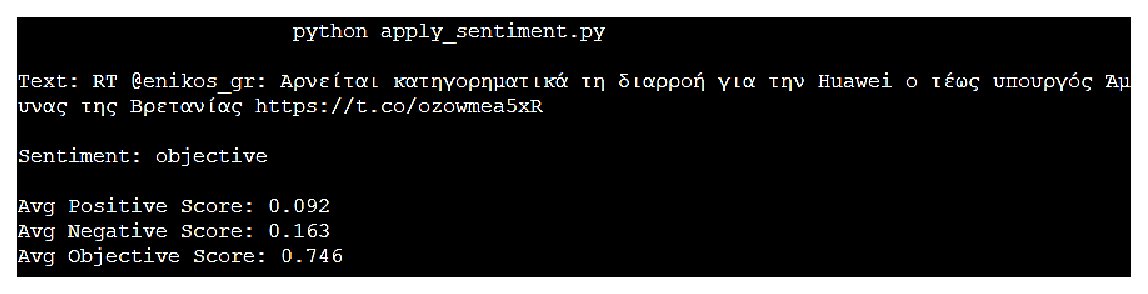
\includegraphics[width=\textwidth]{execution/exec-example.eps}
\caption{Execution Example 1}
\label{fig:exec-example}
\end{figure}

\begin{figure}[ht]
\centering
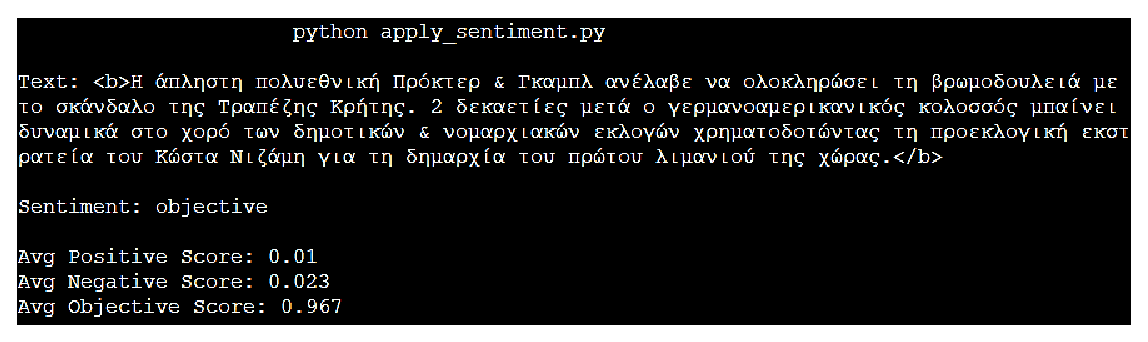
\includegraphics[width=\textwidth]{execution/exec-example2.eps}
\caption{Execution Example 2}
\label{fig:exec-example2}
\end{figure}

\begin{figure}[ht]
\centering
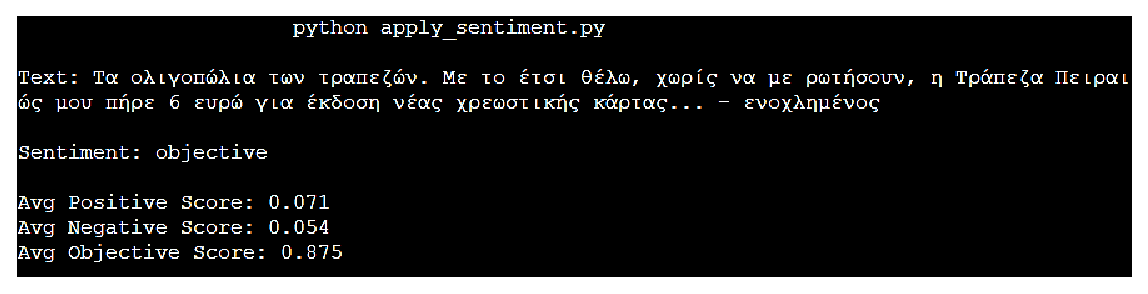
\includegraphics[width=\textwidth]{execution/exec-example3.eps}
\caption{Execution Example 3}
\label{fig:exec-example3}
\end{figure}

\clearpage

\subsubsection{Testing}
\label{subsubsec:testing}

The algorithm was tested on a dataset of 444 Greek posts
of the project of National Bank of Greece.
The particular dataset had initally been annotated with sentiment
through the main algorithm of isMOOD that uses Machine Learning methods,
and then evaluated and corrected by the employees of isMOOD.
The fact that it has been evaluated by human annotators
was critical for its selection,
as it was necessary to have a valid annotated test dataset.

In order to test the algorithm,
the particular dataset was also annotated
through the lexicon-based algorithm that was implemented
as described above.
Then cross-validation was performed between
the initial annotation results
and the ones produced from the new algorithm.
It was found that the rate of agreement of cross-validation
is \textbf{55.91\%}.

The medium rate of agreement is partly explained
by one major issue of SentiWordNet 3.0.
It was noticed that the objective scores
of the terms of SentiWordNet 3.0 are extremely high
compared to the positive and negative scores.
As a result, greek\_sentiment\_terms is composed
of terms with high rates of objectivity,
since it was formed by translating SentiWordNet 3.0.
These high rates of objectivity affect the algorithm;
the words of the input texts receive high objectivity rates,
leading to the texts being mostly annotated as objective.

This issue of the algorithm was not solved during my internship
due to lack of time.
However, there were a few discussions
with my company supervisor and my academic advisor
regarding the solution of this problem.
Two suggestions that resulted from these discussions are the following:

\begin{enumerate}
 \item \emph{Suggestion 1}: Tone down the excessive objectivity
 of greek\_sentiment\_terms
 by dividing the objective scores of all terms with a fixed number,
 and by adding the remaining percentage
 to the positive and negative scores evenly.
 Trial tests were executed for numbers 2 and 3,
 and 3 was found the best option.
 Numbers greater than 3 lead to extreme deduction of objectivity
 to the particular lexicon.
 
 This suggestion is characterised by a considerable bias
 derived from the fact that number 3 is fit to the particular lexicon;
 there is no guarantee that number 3 will be the best option
 for any other lexicon annotated with sentiment.
 
 \item \emph{Suggestion 2}: Append weights to words with higher sensitivity.
 A pre-defined list of words that has been annotated
 by human raters is required,
 in order to recover the most sensitive words.
 
 This suggestion outperforms the first one
 in terms of the bias described above.
 However, multiple human raters are demanded
 to ensure validity for the annotations of the words.
\end{enumerate}
